\section{Processing Setup }\label{sec:methods}
\interfootnotelinepenalty=10000
Using the CVMFS LOFAR software install described in \citep{mechev17}, we processed a typical LOFAR SKSP observation \footnote{LOFAR Observation ID L658492, co-ordinates [17h42m21.785, +037d41m46.805] observed by the LOFAR High Band Array for 8 hours between 2018-06-20 and 2018-06-21. } at multiple different averaging parameters. We test the processing time for different averaging parameters by running 15 runs per parameter step. 

The processing was done on a dedicated node of the SURFsara \texttt{gina} cluster, f18-01. The node is a typical processing node used by our LOFAR Surveys processing, however it is dedicated for the tests in order to ensure there's no contamination by other processes. The specifications of the node are an Intel Xeon 6148 CPU, 384GB RAM and 3TB of scratch (temporary) space. 

There are two sources of latency that need to be studied for a true end-to-end model of LOFAR processing. The first is the performance of the LOFAR software on the Dutch grid for a wide range of processing parameters. The second is the overhead processing, such as job queuing and data movement. We will examine both of these effects in our study of the LOFAR processing performance. While some parts of the processing software may change, the infrastructure parts of our performance model can be used independently of the the processing software and can even be applied to other scientific projects running on the same infrastructure. 

The software pipeline used was the LOFAR \texttt{prefactor} pipeline version used for the LOFAR SKSP broadband surveys \citep{prefactor_zenodo}. 

\subsection{Processing metrics}
The goal for our scalability model is to understand the effect of several parameters on the job completion time of LOFAR software. We do this by testing the slowdown for various values of data size, number of CPUs used and sky model size. 

The data used by the LOFAR surveys is stored at a time resolution of 1 second intervals and frequency resolution of 16 channels per Subband (equivalent to 12kHz channel width). While some of the processing steps such as flagging of Radio Frequency Interference and removal of bright off-axis sources needs to be done on the high-resolution data, later steps can be performed on averaged data. To make processing of these steps more efficient, the raw data is averaged in time and frequency, making the input data size to later tasks smaller. For the LOFAR surveys project, our final averaging parameters are 8 seconds per sample and 2 channels per Subband. This corresponds to a reduction in size by a factor of 64. In section \ref{sec:results_size}, we measure the performance or the \texttt{prefactor} pipeline for data sizes between the raw data of 64GB/Subband and the averaged data of 1GB/Subband. The tested data sizes and parameters are shown in table \ref{table:averaging}. 


\begin{table}[h!]
\centering
\begin{tabular}{||c| c | c | c||} 
 \hline
 Data set & \multicolumn{1}{|p{2cm}|}{\centering Time averaging \\ parameter (sec)} &  \multicolumn{1}{|p{2cm}|}{\centering Channels per Subband} & Size (Gb) \\ [0.5ex]
 \hline
 1GB & 8   & 2   &  1.235   \\ 
 2GB & 4   & 2   &  2.459   \\ 
 4GB & 2   & 2   &  4.906   \\ 
 8GB & 1   & 2   &  9.802   \\ 
 16GB & 1   & 4   &  18.00  \\ 
 32GB & 1   & 8   &  36.72  \\ 
 64GB & 1   & 16   &  66.88  \\[1ex] 
 \hline
\end{tabular}
\caption{Averaging parameters and final data sizes tested for the sample LOFAR SKSP observation. The raw data is 64 GB per Subband. The LOFAR SKSP data processing uses averaging parameters of 8 seconds and 2 channels per Subband. This reduces the raw data by a factor of 64.   }
\label{table:averaging}
\end{table}


The slowest step of the \texttt{prefactor} pipeline is the gsmcal\_solve step, which performs the gain calibration against a model of the radio sky. We obtain this model through the TGSS sky model creator\footnote{Accessible at \href{http://tgssadr.strw.leidenuniv.nl/doku.php}{the TGSS ADR portal}.}. By default this service creates a text sky-model from the TGSS survey \citep{tgssadr} and sets a threshold of sources brighter than 0.3 Jy. Lowering this threshold will typically  create longer sky-model files with more faint sources, while increasing it will return the few brightest sources. Since sky model calibration requires converting the sky-model into UV data \citep{dppp}, a longer sky model will increase the time taken to gain calibrate a data set. We created 7 sky models with minimal flux ranging between 0.05 Jy and 1.5 Jy. The resulting files are listed in Table \ref{table:skymodels}. For production\footnote{The query used to obtain model 3 is \url{http://tgssadr.strw.leidenuniv.nl/cgi-bin/gsmv3.cgi?coord=265.590770833,37.69633472220001\&radius=5\&unit=deg\&deconv=y\&cutoff=0.3 }}, we used the sensitivity parameters for model 3. Each line of these model files corresponds to one source, modelled either as a point or an ellipse), hence the second column also lists the number of sources per sky model file.

It is important to note that the model of the sky depends on the direction of observation. As such, our test is only a heuristic for predicting the run-time based on the sky-model length. The model size and calibration solution quality will differ for other observations and these results will require a further in depth study before changing the calibration strategy. Additionally, it is notable that the number of sources is an exponentially dependent on the minimum sky model sensitivity (seen in Figure \ref{fig:skymodel_size}). According to this relationship, even a modest decrease in sensitivity can significantly decrease the size of the model.

\begin{table}[h!]
\centering
\begin{tabular}{||c| c c||} 
 \hline
 Sky model \# & min sensitivity & \# lines  \\ [0.5ex] 
 \hline
 model 1 & 0.05 Jy & 809    \\ 
 model 2 & 0.1 Jy & 503   \\
 \rowcolor{Gray}
  \hline
 model 3 & 0.3 Jy & 180   \\
  \hline
 model 4 & 0.5 Jy & 96  \\
 model 5 & 0.8 Jy & 49   \\ 
 model 6 & 1.0 Jy & 34   \\
 model 7 & 1.5 Jy & 16   \\[1ex] 
 \hline
\end{tabular}
\caption{List of test sky models. Model 3 is created with the parameters used in our production processing of LOFAR data. All models include objects within 5 degrees from the centre of the pointing.  }
\label{table:skymodels}
\end{table}


\begin{figure}
    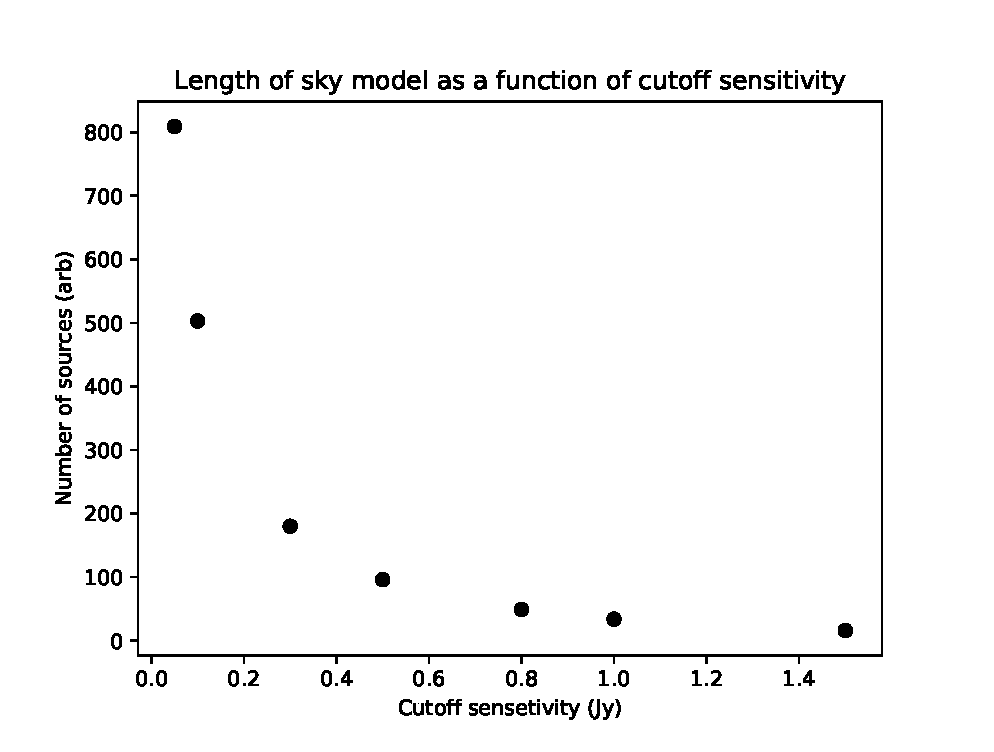
\includegraphics[width=0.95\linewidth]{figures/skymodel_size_vs_Jy.eps}
      \caption{The size of the sky model (measured in number of sources) increases exponentially with the minimum sensitivity of the model.   }
	\label{fig:skymodel_size}
\end{figure}


Finally, the number of CPUs used by each step is a parameter that can be optimized for the entire pipeline. While increasing the number of CPUs can make some steps run faster, requesting jobs that reserve a large number of CPUs will take longer to launch on shared infrastructure. In order to understand these two effects, we study the queuing time and processing time as a function of number of CPUs. For the parameter steps we choose to test 1,2,3,4 8 and 16 CPUs. 

\subsection{Infrastructure performance}
Staging files at different locations can be modelled using historical data, discuss the importance of knowing the time it takes to stage data and the prediction of future performance. 

Since our jobs are launched on a cluster supporting several different use cases, the requested resources are allocated by a job queue, in our case implemented by glite-wms. As queuing jobs can take significant amount of time, we test the queuing time as a function of number of requested CPUs. In order to do that, we create test jobs that log the launch time and submit them, requesting 1, 2, 3, 4, 8 and 16 CPUs. We run several tests for each parameter step to ensure that we capture system variability at different times of day during the week and the weekend. 

Besides queuing, time is also spent during downloading and unpacking data, as well as uploading and packing the results. We measure the time taken to transfer and unpack data of different sizes. The data sizes we chose were 0.5GB, 1GB, 2GB, 4GB, 8GB, 16GB, 32GB and 64GB. As our largest data sets are 64GB and our smallest results are $\sim$0.2GB, these values span a realistic range expected by LOFAR data. We test this by uploading mock data to the dCache storage pool at SURFsara and launching a small 1 CPU job which downloads and untars the data, logging the start time of each step. We present the results of this test in the next section. 


\subsubsection{Software versions}\label{sec:software_versions}
For the current test, we use the LOFAR software stack, version 2.20.2. This software was compiled on a virtual machine and distributed using the CERN CVMFS virtually mounted file system. We use this software version and distribution method as it's the same software version and distribution used to process the data for the LOTSS Data Release 1. 

\subsection{Test Hardware}

The LOFAR software was tested on a reserved node on the SURFsara \texttt{GINA} cluster. The node, f18-01 has 348 GB of RAM, 3TB of scratch space and 40 cores \footnote{More detailed specifications are at \href{http://docs.surfsaralabs.nl/projects/grid/en/latest/Pages/Service/system_specifications/gina_specs.html}{The \texttt{GINA} specification page linked here}}. As this hardware node was reserved, there was no other scientific processing aside from our tests, meaning there was no resource contention aside for that inherent in the LOFAR software. In the results section, we compare these isolated runs with processing results over the past two years. 